{ %%%%%%%%%%%%%%%%%%%%%%%%%%%%%%%%%%%%%%%%%%%
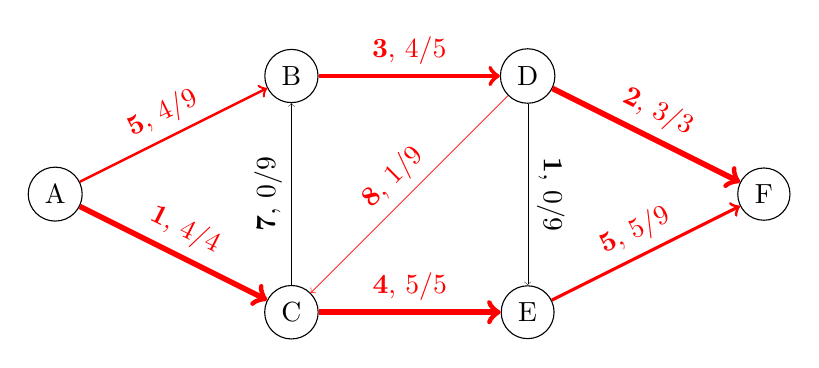
\begin{tikzpicture}

% nodes
\node[draw, circle] at (0,0) (A) {A};
\node[draw, circle] at (3,1.5) (B) {B};
\node[draw, circle] at (3,-1.5) (C) {C};
\node[draw, circle] at (6,1.5) (D) {D};
\node[draw, circle] at (6,-1.5) (E) {E};
\node[draw, circle] at (9,0) (F) {F};

% arcs
\draw [->, line width=0.89pt, red] (A) -- node[above, sloped] {\textbf{5},\ 4/9} (B);
\draw [->, line width=2pt, red] (A) -- node[above, sloped] {\textbf{1},\ 4/4} (C);
\draw [->, line width=1.6pt, red] (B) -- node[above, sloped] {\textbf{3},\ 4/5} (D);
\draw [->, line width=2pt, red] (C) -- node[above, sloped] {\textbf{4}, 5/5} (E);
\draw [->, line width=0.11pt] (C) -- node[above, sloped] {\textbf{7},\ 0/9} (B);
\draw [->, line width=0.22pt, red] (D) -- node[above, sloped] {\textbf{8},\ 1/9} (C);
\draw [->, line width=0.11pt] (D) -- node[above, sloped] {\textbf{1},\ 0/9} (E);
\draw [->, line width=2pt, red] (D) -- node[above, sloped] {\textbf{2},\ 3/3} (F);
\draw [->, line width=1.11pt, red] (E) -- node[above, sloped] {\textbf{5}, 5/9} (F);

\end{tikzpicture}

%\tikz [>=spaced stealth']
%\tikz
%\graph [spring layout, edge quotes mid, grow=right, nodes={draw, circle},
%        node distance=2cm, horizontal=B to D, vertical=B to C,
%        edges={nodes={font=\scriptsize, fill=white, sloped, inner sep=1pt}}]
%{
%  A ->[red, line width=2pt] B,
%  A ->[red, very thick] C,
%  B -> D,
%  B ->[red, very thick] E,
%  C -> B,
%  C ->[red, very thick] E,
%  D -> C,
%  D ->[red, very thick] F,
%  E ->[red, very thick] D,
%  E ->[red, very thick] F,
%};
%  { A ->[bend left, red] B }
} %%%%%%%%%%%%%%%%%%%%%%%%%%%%%%%%%%%%%%%%%%%

